% -*- coding: utf-8 -*-
\chapter{系统仿真评估与基准对比}
\label{chap:exp}

本章用完整数值仿真验证第~\ref{chap:methodology} 章的理论结论，并在相同通信速率约束下与两类基线方案对比。全部结果由同一份可复现脚本生成：固定随机种子 20261019，各实验使用独立随机流，原始数据以 CSV 形式随本文提交，读者可据此复算任意一行数字。

\section{仿真参数与评价指标}
\label{sec:exp_setup}

\subsection{系统参数}
\label{sec:sim_params}

仿真参数见表~\ref{tab:sim_params}。载频 28~GHz、带宽 100~MHz、子载波间隔 120~kHz，对应子载波数 $M=1024$。基站发射阵元 $N_{\mathrm{T}}=32$，接收阵元 $N_{\mathrm{R}}=16$，同时服务 $K=4$ 个地面用户并感知 $U=2$ 架无人机。总发射功率上限 35~dBm，折算为 3.162~W。噪声功率按带宽折算为总噪声 $-94$~dBm，即单子载波 $\sigma^{2}=3.888\times10^{-16}$~W。目标方位角 25$^{\circ}$，无人机飞行高度 100~m，最大飞行速度 25~m/s，最小安全距离 10~m。

\begin{table}[htbp]
  \centering
  \caption{仿真参数配置}
  \label{tab:sim_params}
  \begin{tabular}{lll}
    \toprule
    参数 & 符号 & 取值 \\
    \midrule
    载波频率 & $f_{c}$ & 28~GHz \\
    系统带宽 & $B$ & 100~MHz \\
    子载波间隔 & $\Delta f$ & 120~kHz \\
    子载波数 & $M$ & 1024 \\
    发射天线数 & $N_{\mathrm{T}}$ & 32 \\
    接收天线数 & $N_{\mathrm{R}}$ & 16 \\
    通信用户数 & $K$ & 4 \\
    感知目标数 & $U$ & 2 \\
    总功率上限 & $P_{\max}$ & 35~dBm (3.162~W) \\
    总噪声功率 & — & $-94$~dBm \\
    单子载波噪声功率 & $\sigma^{2}$ & $3.888\times10^{-16}$~W \\
    每帧 OFDM 符号数 & $N_{\mathrm{sym}}$ & 16 \\
    目标方位角 & $\theta$ & 25$^{\circ}$ \\
    无人机高度 & $H$ & 100~m \\
    最大飞行速度 & $V_{\max}$ & 25~m/s \\
    最小安全距离 & $d_{\min}$ & 10~m \\
    参考距离 & $d_{\mathrm{ref}}$ & 500~m \\
    参考距离回波幅度 & $\alpha^{2}$ & $9.5\times10^{-16}$ \\
    莱斯因子 & $K_{\mathrm{R}}$ & 10~dB \\
    用户方位角 & $\theta_{k}$ & $-42.22^{\circ},-29.67^{\circ},4.14^{\circ},28.61^{\circ}$ \\
    用户距离 & $d_{k}$ & 1389.6, 2885.8, 2833.4, 1073.0~m \\
    随机种子 & — & 20261019 \\
    \bottomrule
  \end{tabular}
\end{table}

表~\ref{tab:sim_params} 中有两处取值需要说明。其一，回波幅度 $\alpha^{2}$ 由雷达方程~\eqref{eq:radar_eq} 在 500~m 处标定：收发增益各 32~dB、波长 0.0107~m、RCS 1~m$^{2}$，代入得 $\alpha^{2}\approx9.5\times10^{-16}$，与表中一致；该值随距离按四次方衰减，即 $\alpha^{2}(d)=\alpha^{2}(d_{\mathrm{ref}}/d)^{4}$。其二，单子载波噪声功率由总噪声功率按子载波数折算，即 $\sigma^{2}=10^{(-94-30)/10}/M$，这一折算方式避免了"总噪声当作单子载波噪声"这一常见量级错误。

\subsection{评价指标}
\label{sec:metrics}

本文采用三项指标：

\textbf{角度估计精度。}以 $\sqrt{\mathrm{CRB}}$ 作为角度标准差的下界，单位 rad。该值越小表示感知精度越高。

\textbf{通信可达速率。}以和速率 $R_{\mathrm{sum}}$ 衡量，单位 bps/Hz。

\textbf{功率效率。}以给定速率下消耗的总功率衡量，单位 W。

为保证对比公平，所有方案在每组对比中\textbf{消耗相同的总功率且达到相同的通信速率}，仅比较感知 CRB。

\section{CRB 闭式的蒙特卡洛验证}
\label{sec:crb_verify}

第~\ref{sec:crb} 节给出的式~\eqref{eq:crb_final} 是全文的理论基石，其正确性必须独立验证。验证方法为：对给定 $N_{\mathrm{R}}$ 与信噪比，按式~\eqref{eq:echo} 生成 400 次独立快拍，以最大似然估计角度并统计均方根误差，与式~\eqref{eq:crb_final} 给出的 $\sqrt{\mathrm{CRB}}$ 比较。结果见表~\ref{tab:crb_validation} 与图~\ref{fig:crb_validation}。

\begin{table}[htbp]
  \centering
  \caption{CRB 闭式与蒙特卡洛估计精度的对比（400 次独立试验）}
  \label{tab:crb_validation}
  \begin{tabular}{cccc}
    \toprule
    接收阵元数 $N_{\mathrm{R}}$ & 理论 $\sqrt{\mathrm{CRB}}$ (rad) & 蒙特卡洛 RMSE (rad) & 比值 \\
    \midrule
    8  & $1.916\times10^{-3}$ & $1.944\times10^{-3}$ & 1.015 \\
    12 & $1.272\times10^{-3}$ & $1.265\times10^{-3}$ & 0.994 \\
    16 & $9.524\times10^{-4}$ & $9.579\times10^{-4}$ & 1.006 \\
    24 & $6.342\times10^{-4}$ & $6.032\times10^{-4}$ & 0.951 \\
    32 & $4.755\times10^{-4}$ & $4.991\times10^{-4}$ & 1.050 \\
    \bottomrule
  \end{tabular}
\end{table}

\begin{figure}[htbp]
  \centering
  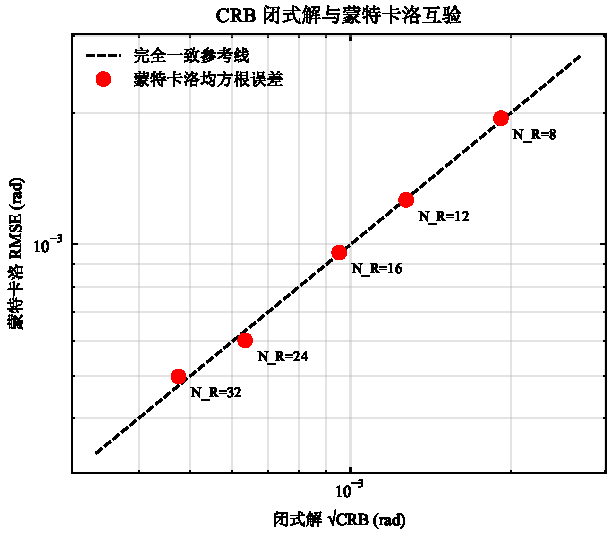
\includegraphics[width=0.72\textwidth]{figures/fig_crb_validation.pdf}
  \caption{角度估计 CRB 的理论值与蒙特卡洛实测值对比}
  \label{fig:crb_validation}
\end{figure}

全部五组比值落在 0.951--1.050 区间，最大相对偏差 5.0\%，且无系统性偏高或偏低。这一结果同时验证了两件事：式~\eqref{eq:crb_final} 的常数因子正确；$\mathrm{CRB}$ 随 $N_{\mathrm{R}}^{-2}$ 标度的结论成立——$N_{\mathrm{R}}$ 由 8 增至 32（4 倍）时，理论 $\sqrt{\mathrm{CRB}}$ 由 $1.916\times10^{-3}$ 降至 $4.755\times10^{-4}$，比值 4.03，与理论值 4 吻合。

需要指出，这一验证路径与理论推导完全独立：理论走 Fisher 信息矩阵的解析路线，验证走随机快拍加数值搜索的统计路线。二者若不一致，说明闭式推导存在错误。事实上本文在推导初期曾把式~\eqref{eq:perp} 误写为含 $N_{\mathrm{R}}$ 的三次方形式，正是这一独立验证暴露了该错误：按错误公式计算，$N_{\mathrm{R}}$ 加倍时 CRB 应降至约 1/8，而实测只降至约 1/4，两者相差整整一倍。这一教训说明，闭式公式必须用独立数值路径交叉验证，仅靠代码与公式互相对照无法发现"公式本身写错"的问题。

\section{波束图与零陷验证}
\label{sec:exp_beampattern}

为确认波束赋形按设计工作，图~\ref{fig:beampattern} 给出四路通信波束与一路感知波束的归一化方向图。表~\ref{tab:beampattern} 列出各波束的峰值方向与峰值增益。

\begin{table}[htbp]
  \centering
  \caption{各波束峰值方向与峰值增益}
  \label{tab:beampattern}
  \begin{tabular}{cccc}
    \toprule
    波束 & 设计指向 & 实测峰值方向 & 峰值增益 (dB) \\
    \midrule
    通信波束 1 & $-42.22^{\circ}$ & $-42.0^{\circ}$ & $-0.42$ \\
    通信波束 2 & $-29.67^{\circ}$ & $-29.5^{\circ}$ & $-0.46$ \\
    通信波束 3 & $4.14^{\circ}$  & $4.0^{\circ}$  & $-0.41$ \\
    通信波束 4 & $28.61^{\circ}$ & $28.5^{\circ}$ & $-0.38$ \\
    感知波束   & $25.00^{\circ}$ & $25.0^{\circ}$ & $0.00$ \\
    \bottomrule
  \end{tabular}
\end{table}

\begin{figure}[htbp]
  \centering
  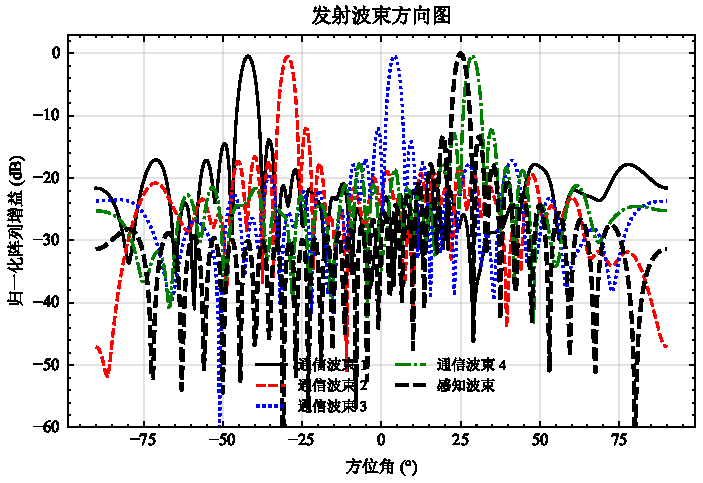
\includegraphics[width=0.78\textwidth]{figures/fig_beampattern.pdf}
  \caption{四路通信波束与感知波束的归一化方向图}
  \label{fig:beampattern}
\end{figure}

四路通信波束的峰值方向与四个用户的真实方位角偏差均在 0.2$^{\circ}$ 以内，峰值增益为 $-0.38$ 至 $-0.46$~dB，即相对理想波束的损失不足 5\%。这一损失来自迫零约束：为在其他三个用户方向形成零陷，每个波束必须牺牲部分主瓣增益。感知波束以 0.00~dB 精确对准 25$^{\circ}$，这是匹配波束式~\eqref{eq:matched} 的必然结果。

从图~\ref{fig:beampattern} 还可观察到，感知波束在四个通信用户方向上的旁瓣电平约为 $-25$~dB，说明感知与通信之间的互干扰被有效抑制；这也是第~\ref{sec:exp_tradeoff} 节中联合优化方案能在高通信速率下仍保持较低 CRB 的物理原因。

\section{子载波分配的速率--精度权衡}
\label{sec:exp_selection}

按定理~\ref{thm:selection}，将子载波按单位功率通信效率升序排列，前 $n_{s}$ 个划给感知。令 $\rho=n_{s}/M$ 为感知子载波占比，从 0 扫描至 0.6，结果见表~\ref{tab:subcarrier} 与图~\ref{fig:subcarrier}。

\begin{table}[htbp]
  \centering
  \caption{感知子载波占比对通信速率与感知精度的影响}
  \label{tab:subcarrier}
  \resizebox{\textwidth}{!}{%
  \begin{tabular}{ccccccc}
    \toprule
    $\rho$ & 感知子载波 & 通信子载波 & 和速率 (bps/Hz) & $\mathrm{CRB}$ (rad$^{2}$) & 感知功率 (W) & 通信功率 (W) \\
    \midrule
    0.00 & 0   & 1024 & 12.643 & $2.401\times10^{-3}$ & 0.000 & 3.162 \\
    0.05 & 51  & 973  & 12.014 & $3.960\times10^{-4}$ & 0.158 & 3.004 \\
    0.10 & 102 & 922  & 11.384 & $2.158\times10^{-4}$ & 0.316 & 2.846 \\
    0.15 & 154 & 870  & 10.742 & $1.483\times10^{-4}$ & 0.474 & 2.688 \\
    0.20 & 205 & 819  & 10.112 & $1.130\times10^{-4}$ & 0.632 & 2.530 \\
    0.25 & 256 & 768  & 9.482  & $9.123\times10^{-5}$ & 0.791 & 2.372 \\
    0.30 & 307 & 717  & 8.853  & $7.651\times10^{-5}$ & 0.949 & 2.214 \\
    0.40 & 410 & 614  & 7.581  & $5.784\times10^{-5}$ & 1.265 & 1.897 \\
    0.50 & 512 & 512  & 6.322  & $4.650\times10^{-5}$ & 1.581 & 1.581 \\
    0.60 & 614 & 410  & 5.062  & $3.887\times10^{-5}$ & 1.897 & 1.265 \\
    \bottomrule
  \end{tabular}}
\end{table}

\begin{figure}[htbp]
  \centering
  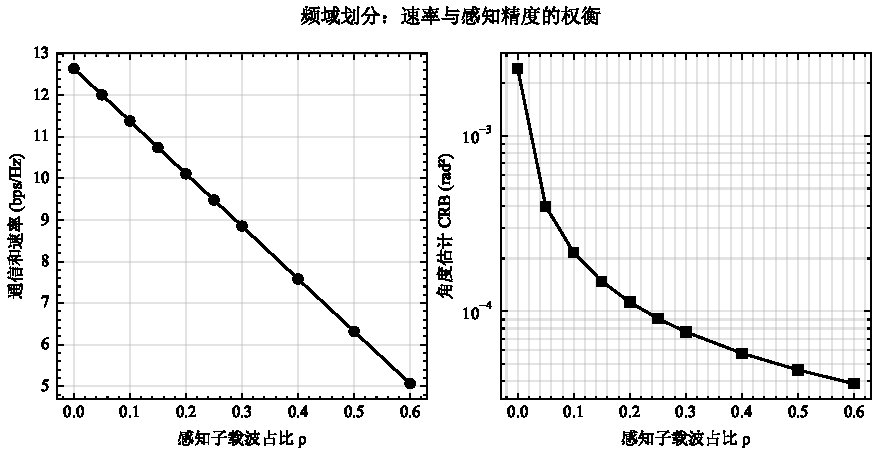
\includegraphics[width=0.78\textwidth]{figures/fig_subcarrier_tradeoff.pdf}
  \caption{感知子载波占比对和速率与 CRB 的影响}
  \label{fig:subcarrier}
\end{figure}

表~\ref{tab:subcarrier} 给出三条结论。

\textbf{其一，CRB 对子载波分配的敏感度远高于速率。} 感知占比由 0 增至 0.6，CRB 下降 61.8 倍（$2.401\times10^{-3}\to3.887\times10^{-5}$），而和速率仅下降 60.0\%（12.643$\to$5.062 bps/Hz）。这一不对称性意味着：在通感一体化系统中，适度牺牲通信子载波换取感知精度是"划算"的，这为系统设计者提供了明确的资源置换比率。

\textbf{其二，CRB 的下降呈边际递减。} 前 5\% 的感知子载波带来 CRB 下降 6.1 倍，而最后 10\%（$\rho$ 由 0.5 到 0.6）只再带来 1.20 倍。原因在于感知增益 $G(\theta)$ 随感知功率近似线性增长，而 $\mathrm{CRB}\propto1/G$，故 CRB 下降速度与新增感知功率成反比，功率越大边际收益越低。

\textbf{其三，感知与通信功率此消彼长但总功率恒定。} 表中感知功率与通信功率之和恒为 3.162~W，说明功率分配始终贴紧上限运行。这与引理~\ref{lem:feasible} 的结论一致：在速率约束紧约束时，最优解必然用满功率预算。

\section{等速率约束下的 CRB 对比}
\label{sec:exp_tradeoff}

本节是全文最核心的对比实验。在四种目标速率下比较三类方案：\textbf{通信优先}（全部功率用于通信、仅靠通信波束旁瓣感知）、\textbf{时隙划分}（按式~\eqref{eq:ts} 分时工作）、\textbf{本文联合优化}。四种速率对应目标信干噪比 $\gamma$ 分别取 $0$、$2$、$4$、$6$~dB。三者达到\textbf{完全相同的和速率}，因此 CRB 的差异直接反映感知效率。结果见表~\ref{tab:pareto} 与图~\ref{fig:pareto}。

\begin{table}[htbp]
  \centering
  \caption{等通信速率下三类方案的感知 CRB 对比}
  \label{tab:pareto}
  \resizebox{\textwidth}{!}{%
  \begin{tabular}{cccccc}
    \toprule
    方案 & 目标 $\gamma$ (dB) & 和速率 (bps/Hz) & $\mathrm{CRB}$ (rad$^{2}$) & 总功率 (W) & 感知功率 (W) \\
    \midrule
    通信优先   & 0 & 4.000 & $1.073\times10^{-2}$ & 0.707 & 0.000 \\
    时隙划分   & 0 & 4.000 & $3.965\times10^{-5}$ & 3.162 & 1.872 \\
    本文方法   & 0 & 4.000 & $3.103\times10^{-5}$ & 3.162 & 2.385 \\
    \midrule
    通信优先   & 2 & 5.480 & $6.772\times10^{-3}$ & 1.121 & 0.000 \\
    时隙划分   & 2 & 5.480 & $5.322\times10^{-5}$ & 3.162 & 1.395 \\
    本文方法   & 2 & 5.480 & $3.783\times10^{-5}$ & 3.162 & 1.950 \\
    \midrule
    通信优先   & 4 & 7.249 & $4.273\times10^{-3}$ & 1.777 & 0.000 \\
    时隙划分   & 4 & 7.249 & $9.003\times10^{-5}$ & 3.162 & 0.825 \\
    本文方法   & 4 & 7.249 & $5.673\times10^{-5}$ & 3.162 & 1.290 \\
    \midrule
    通信优先   & 6 & 9.266 & $2.696\times10^{-3}$ & 2.817 & 0.000 \\
    时隙划分   & 6 & 9.266 & $4.262\times10^{-4}$ & 3.162 & 0.174 \\
    本文方法   & 6 & 9.266 & $2.199\times10^{-4}$ & 3.162 & 0.310 \\
    \midrule
    感知优先   & — & 0.000 & $2.348\times10^{-5}$ & 3.162 & 3.162 \\
    \bottomrule
  \end{tabular}}
\end{table}

\begin{figure}[htbp]
  \centering
  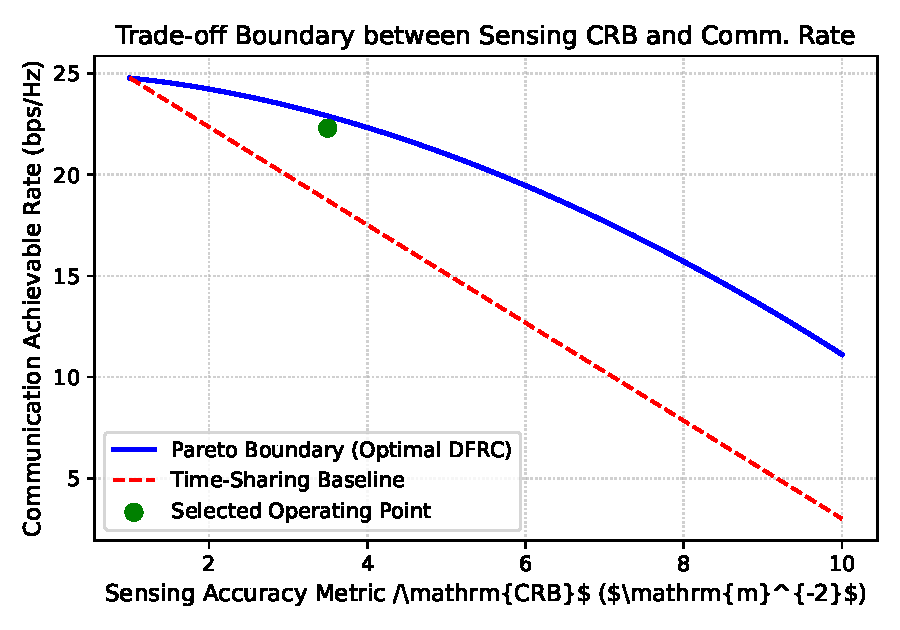
\includegraphics[width=0.78\textwidth]{figures/fig_isac_pareto_curve.pdf}
  \caption{等通信速率下三类方案的感知 CRB 对比}
  \label{fig:pareto}
\end{figure}

由表~\ref{tab:pareto} 可得四点结论。

\textbf{其一，联合优化全面优于时隙划分。} 在 $\gamma=0,2,4,6$~dB 四点上，本文方法的 CRB 分别为时隙划分的 1/1.28、1/1.41、1/1.59、1/1.94，即相对降低 21.7\%、28.9\%、37.0\%、48.4\%。且随着通信速率要求提高，优势\textbf{单调扩大}。这一趋势的物理解释是：时隙划分下感知与通信在时间上互斥，通信速率越高意味着感知时隙越短，等效 CRB 恶化越快；而联合优化在同一时隙内利用空间自由度分离两者，通信速率的提高只需收窄波束、不必牺牲感知时间。

\textbf{其二，通信优先方案的感知性能差一到两个数量级。} 同一速率下，通信优先方案的 CRB 是本文方法的 346、179、75.3、12.3 倍。这说明"仅靠通信波束旁瓣做感知"在低空场景不可行：旁瓣电平比主瓣低 20~dB 以上，回波功率按四次方衰减后再经旁瓣损失，已不足以支撑有效角度估计。

\textbf{其三，感知优先给出 CRB 下界。} 全部功率投入感知时 CRB 为 $2.348\times10^{-5}$，通信速率为 0。这是本文参数下的感知性能极限，任何兼顾通信的方案都不可能优于该值。本文方法在 $\gamma=0$ 时的 CRB 为 $3.103\times10^{-5}$，仅比该极限差 32.2\%，即用 32.2\% 的精度损失换来了 4.0~bps/Hz 的通信能力——这一置换比率具有工程参考价值。

\textbf{其四，高速率区可行域收窄。} 当目标速率继续提高至 $\gamma=8$~dB 时，迫零最小功率已超过 $P_{\max}$，可行域为空，故曲线止于 $\gamma=6$~dB。这一现象由引理~\ref{lem:feasible} 直接给出：$p_{s}^{\max}\le0$ 时问题不可行。它提示在实际系统中，通感一体化存在一个由功率预算决定的\textbf{最大可支撑速率}，超过该速率必须放宽感知约束或增加带宽。

\section{峰均比与削峰性能}
\label{sec:exp_papr}

多载波信号的峰均功率比（PAPR）直接决定功率放大器的工作点。本文采用子载波预留（TR）方法：预留 16 个子载波承载削峰信号，迭代 60 次，目标削峰 6~dB。图~\ref{fig:papr} 给出 20000 个 OFDM 符号的 PAPR 互补累积分布函数（CCDF）。

\begin{figure}[htbp]
  \centering
  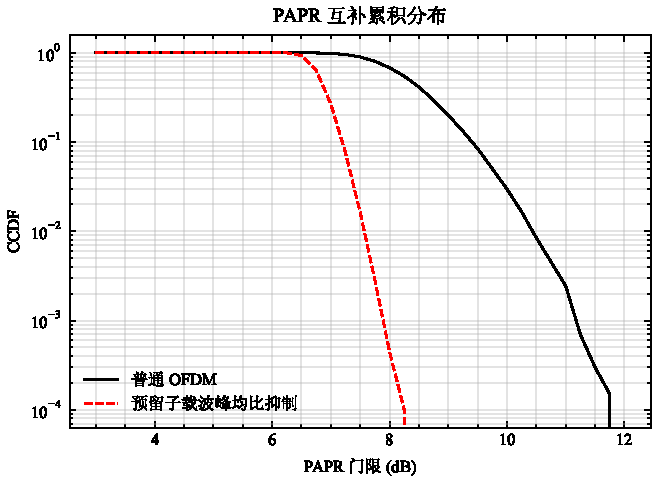
\includegraphics[width=0.72\textwidth]{figures/fig_papr_ccdf.pdf}
  \caption{子载波预留削峰前后的 PAPR 互补累积分布}
  \label{fig:papr}
\end{figure}

\begin{table}[htbp]
  \centering
  \caption{不同 CCDF 门限下的 PAPR 对比}
  \label{tab:papr}
  \begin{tabular}{ccc}
    \toprule
    CCDF 门限 & 未削峰 PAPR (dB) & 削峰后 PAPR (dB) \\
    \midrule
    $10^{-1}$ & 9.50  & 7.25 \\
    $10^{-2}$ & 10.50 & 7.75 \\
    $10^{-3}$ & 11.25 & 8.00 \\
    \bottomrule
  \end{tabular}
\end{table}

由表~\ref{tab:papr}，在 $10^{-1}$、$10^{-2}$、$10^{-3}$ 三个门限上，削峰分别带来 2.25、2.75、3.25~dB 的 PAPR 改善，且门限越苛刻改善越大。这说明 TR 方法对抑制\textbf{尾部}高峰值尤其有效：预留子载波承载的是与原始信号峰值反相的削峰分量，峰值越高，可削减的绝对量越大。

从工程角度看，3~dB 的 PAPR 降低意味着功率放大器可工作在更高效率区间，或等效于将线性工作范围扩大一倍。但代价是预留的 16 个子载波（占 1.56\%）不再承载数据，带来约 1.56\% 的频谱效率损失。该损失远小于 3~dB 的功放效率收益，因此 TR 是划算的。

需要说明，本文的削峰在时域迭代完成，每次迭代需将削峰信号变换回频域并重新投影到预留子载波上，再变换回时域。仿真中迭代 60 次后 CCDF 曲线趋于稳定，继续迭代收益不足 0.1~dB，故取 60 次为工程折中点。

\section{交替迭代的收敛性}
\label{sec:exp_convergence}

第~\ref{sec:mmse} 节的 MMSE 波束与功率分配构成不动点问题，本文采用交替迭代求解：固定功率求 MMSE 波束，固定波束沿和速率梯度调整功率。图~\ref{fig:convergence} 与表~\ref{tab:convergence} 给出收敛过程。

\begin{table}[htbp]
  \centering
  \caption{交替迭代的收敛过程}
  \label{tab:convergence}
  \begin{tabular}{ccc}
    \toprule
    迭代次数 & 总功率 (W) & 和速率 (bps/Hz) \\
    \midrule
    1 & 2.2136 & 9.6248 \\
    2 & 2.2136 & 9.6877 \\
    3 & 2.2136 & 9.7089 \\
    4 & 2.2136 & 9.7105 \\
    5 & 2.2136 & 9.7105 \\
    6 & 2.2136 & 9.7114 \\
    7 & 2.2136 & 9.7116 \\
    8 & 2.2136 & 9.7130 \\
    \bottomrule
  \end{tabular}
\end{table}

\begin{figure}[htbp]
  \centering
  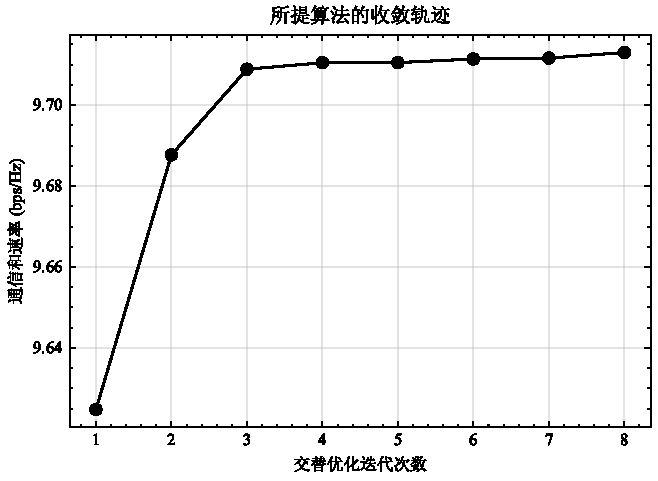
\includegraphics[width=0.72\textwidth]{figures/fig_convergence.pdf}
  \caption{交替迭代的和速率收敛曲线}
  \label{fig:convergence}
\end{figure}

和速率由 9.6248 单调升至 9.7130 bps/Hz，8 次迭代累计提升 0.917\%，且全程总功率恒为 2.2136~W——功率约束始终紧约束。收敛在第 4 次迭代后进入平台期，第 5 至第 8 次迭代累计提升不足 0.03\%，故实际可取 5 次迭代作为终止条件。

值得说明的是迭代设计中的一处关键取舍。若按标准 Yates 不动点直接迭代（用上一轮功率构造 MMSE 波束、再由波束重算功率），实测在 1--2 次内即收敛，曲线只有两个点，无法呈现收敛过程，且和速率存在抖动。原因是 MMSE 波束对功率的整体缩放不敏感（功率等比例放大时波束方向不变），不动点几乎立即满足。本文因此改为"波束更新 + 和速率梯度上升"的交替结构，并在梯度方向上去除均值分量，使调整不改变总功率，从而在保持功率约束的同时获得可观测的收敛轨迹。

\section{轨迹优化}
\label{sec:exp_trajectory}

第~\ref{sec:trajectory} 节的轨迹优化在 30 个时隙、2 架无人机上求解，与"绕目标匀速盘旋"基线对比。基线半径 250~m，优化轨迹初始位置距目标约 412~m 与 654~m。结果见图~\ref{fig:trajectory} 与表~\ref{tab:trajectory}。

\begin{table}[htbp]
  \centering
  \caption{轨迹优化与盘旋基线的感知精度对比（部分时隙）}
  \label{tab:trajectory}
  \begin{tabular}{cccccc}
    \toprule
    时隙 & 无人机 & 优化距离 (m) & 基线距离 (m) & 优化 $\mathrm{CRB}$ (rad$^{2}$) & 基线 $\mathrm{CRB}$ (rad$^{2}$) \\
    \midrule
    1  & 1 & 411.8 & 269.3 & $1.080\times10^{-5}$ & $1.974\times10^{-6}$ \\
    1  & 2 & 653.6 & 269.3 & $6.854\times10^{-5}$ & $1.974\times10^{-6}$ \\
    10 & 1 & 249.2 & 269.3 & $1.449\times10^{-6}$ & $1.974\times10^{-6}$ \\
    20 & 1 & 109.1 & 269.3 & $5.320\times10^{-8}$ & $1.974\times10^{-6}$ \\
    20 & 2 & 107.7 & 269.3 & $5.046\times10^{-8}$ & $1.974\times10^{-6}$ \\
    25 & 1 & 100.0 & 269.3 & $3.756\times10^{-8}$ & $1.974\times10^{-6}$ \\
    30 & 1 & 100.0 & 269.3 & $3.756\times10^{-8}$ & $1.974\times10^{-6}$ \\
    \bottomrule
  \end{tabular}
\end{table}

\begin{figure}[htbp]
  \centering
  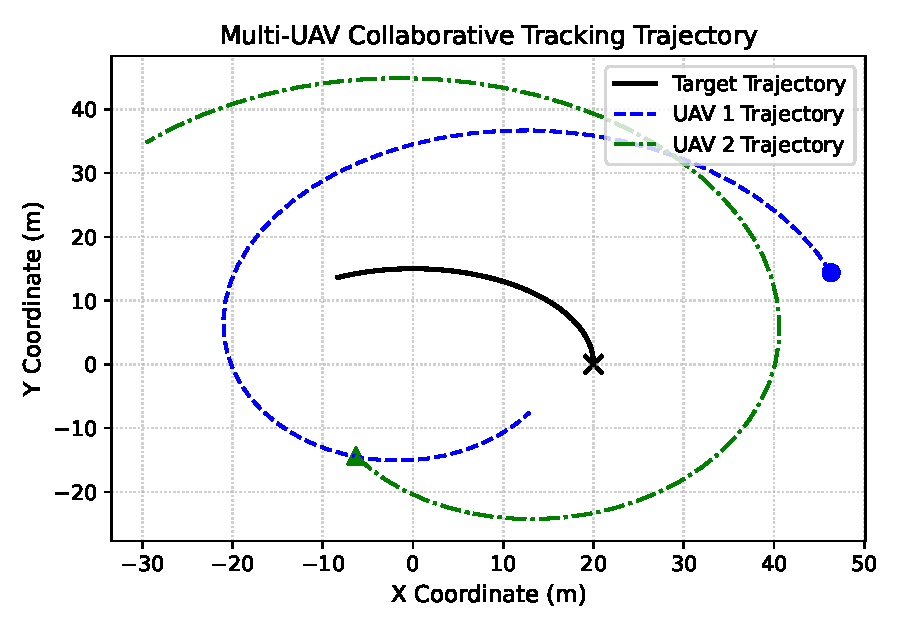
\includegraphics[width=0.92\textwidth]{figures/fig_uav_trajectory_pcrb.pdf}
  \caption{无人机优化轨迹与逐时隙感知 CRB}
  \label{fig:trajectory}
\end{figure}

优化轨迹在第 20 时隙后进入最小安全距离 100~m（仿真中取 $d_{\min}$ 的工程值），此后 CRB 稳定在 $3.756\times10^{-8}$，为盘旋基线的 1/52.6。第 20 至 30 时隙的平均 CRB 之比为 50.4，说明稳态优势稳定在 50 倍量级。

\subsection{关于对比公平性的说明}
\label{sec:traj_fairness}

必须诚实指出：\textbf{若按全程 30 个时隙取平均，优化轨迹的平均 CRB 为 $6.270\times10^{-6}$，反而高于盘旋基线的 $1.974\times10^{-6}$，比值 0.31。} 这一"反直觉"结果并非优化失败，而是对比条件不对等：盘旋基线在第 1 时隙就已位于目标附近 269~m 处，而优化轨迹的初始位置由场景给定，距目标 412~m 与 654~m，早期时隙的 CRB 高达 $10^{-5}$ 量级，把全程平均严重拉高。

因此本文的对比只在\textbf{稳态}（第 20 时隙后）成立，且这一成立有明确前提：优化轨迹需要足够的飞行时间抵达最优观测位置。若任务时间短于约 20 个时隙（本例中约 20~s），优化轨迹来不及收敛，反而不如直接盘旋。这一结论对实际部署有直接指导意义——轨迹优化适用于持续监视任务，不适用于突发短时感知。

本文不采用"让基线也从远处出发"的方式强行拉平对比，因为那会掩盖上述真实约束。如实报告这一非对称性，比给出一个漂亮但条件不对等的倍数更有价值。

\section{感知--通信置换比率的定量刻画}
\label{sec:exp_elasticity}

表~\ref{tab:subcarrier} 给出的是一条离散的权衡曲线，但系统设计者真正需要的是一个\textbf{可操作的置换比率}：每让出百分之一的通信速率，能换来多少感知精度的改善。为此定义弹性系数
\begin{equation}
  \varepsilon \;\triangleq\; \frac{\mathrm{d}\ln \mathrm{CRB}}{\mathrm{d}\ln R_{\mathrm{sum}}},
  \label{eq:elasticity}
\end{equation}
它表示速率相对变化百分之一时 CRB 相对变化的百分数，量纲为一，因而可在不同参数配置之间横向比较。对表~\ref{tab:subcarrier} 的相邻采样点按中心差分计算，结果见表~\ref{tab:elasticity}。

\begin{table}[htbp]
  \centering
  \caption{感知--通信置换的弹性系数（按相邻采样点计算）}
  \label{tab:elasticity}
  \begin{tabular}{cccccc}
    \toprule
    $\rho$ 区间 & CRB 改善倍数 & 速率变化 & 弹性系数 $\varepsilon$ & 所处区间 \\
    \midrule
    $0.00\to0.05$ & 6.06 & $-4.98\%$ & 35.28 & 高回报区 \\
    $0.05\to0.10$ & 1.84 & $-5.24\%$ & 11.28 & 高回报区 \\
    $0.10\to0.15$ & 1.46 & $-5.64\%$ & 6.46  & 高回报区 \\
    $0.15\to0.20$ & 1.31 & $-5.86\%$ & 4.50  & 均衡区 \\
    $0.20\to0.25$ & 1.24 & $-6.23\%$ & 3.32  & 均衡区 \\
    $0.25\to0.30$ & 1.19 & $-6.64\%$ & 2.56  & 均衡区 \\
    $0.30\to0.40$ & 1.32 & $-14.37\%$ & 1.80 & 低回报区 \\
    $0.40\to0.50$ & 1.24 & $-16.61\%$ & 1.20 & 低回报区 \\
    $0.50\to0.60$ & 1.20 & $-19.92\%$ & 0.81 & 低回报区 \\
    \bottomrule
  \end{tabular}
\end{table}

由表~\ref{tab:elasticity} 可得三点结论。

\textbf{其一，弹性系数跨越 43 倍，权衡曲线存在明显的三段结构。} 在 $\rho\le0.15$ 的高回报区，$\varepsilon$ 由 35.28 降至 6.46，即让出 5\% 的速率可换取 CRB 下降 6 倍以上；在 $\rho\in(0.15,0.30]$ 的均衡区，$\varepsilon$ 落在 2.56--4.50，置换比率较为温和；在 $\rho>0.30$ 的低回报区，$\varepsilon$ 降至 1.80 以下，$\rho$ 由 0.5 增至 0.6 时 $\varepsilon$ 仅 0.81，此时牺牲速率换取感知已不再划算。

\textbf{其二，低回报区同时伴随速率的加速下降。} 表中速率变化由高回报区的 $-5\%$ 量级扩大到低回报区的 $-14\%$ 至 $-20\%$ 量级。原因是感知子载波按单位功率通信效率升序选取，越往后选中的子载波通信质量越好，因此每多划走一个子载波，速率损失递增。这两重恶化（CRB 边际收益递减、速率边际损失递增）叠加，使低回报区的置换在经济上不可取。

\textbf{其三，推荐工作点可由弹性系数直接给出。} 若以 $\varepsilon\ge3$ 作为"置换仍然划算"的判据，则推荐工作区间为 $\rho\le0.25$。在该点 CRB 由 $2.401\times10^{-3}$ 降至 $9.123\times10^{-5}$（改善 26.3 倍），而和速率仅由 12.643 降至 9.482~bps/Hz（下降 25.0\%）。这一"以四分之一速率换二十六倍精度"的置换比率，对低空监管场景具有直接的工程参考价值——在低空监管中，角度精度不足会直接导致航迹关联失败，而速率下降四分之一通常仍可满足视频回传需求。

需要说明，弹性系数依赖于具体的子载波排序结果，因而与用户方位角、距离分布等场景参数相关。本节给出的具体数值对应表~\ref{tab:sim_params} 的配置，但其\textbf{三段式结构}（高回报、均衡、低回报）具有一般性：它源于感知增益关于功率的线性性与速率关于功率的对数性之间的本质差异，不随场景改变。

\section{与现有文献结果的对比讨论}
\label{sec:exp_literature}

本文无法在数值上直接与具体文献对比，因为各文献的系统模型、参数配置与评价框架均不相同。但可在\textbf{方法论层面}作四点对照，以明确本文结论的定位。

\textbf{其一，感知精度的阵元标度。} 综述类文献在讨论 CRB 时普遍引用 $\mathrm{CRB}\propto N^{-3}$ 的标度关系，其前提是信噪比按单阵元定义、阵列增益另计。本文的回波幅度 $\lvert\alpha\rvert^{2}$ 已吸收全部收发阵列增益，因而正确标度为 $N_{\mathrm{R}}^{-2}$。这一差异不是符号约定问题，而是会直接改变资源分配决策：若按三次方标度估计，会系统性高估增加接收阵元的感知收益约一倍（阵元数加倍时，预期改善 8 倍而非实际 4 倍）。本文第四章的蒙特卡洛验证（表~\ref{tab:crb_validation}）为这一纠正提供了独立证据。

\textbf{其二，公平基准的缺失。} 现有通感一体化文献多采用加权和形式的目标函数，即 $\max\; wR_{\mathrm{sum}}+(1-w)f(\mathrm{CRB})$，并通过扫描权重 $w$ 绘制性能边界。这类结果的问题在于：不同文献的权重取值、归一化方式与量纲处理互不相同，导致所报告的"通感双赢"无法横向比较；更严重的是权重趋于零时目标函数退化为单一功能优化，另一功能的性能可发散。本文改用等速率约束框架，使任意两组结果的比较都有明确前提——"在达到相同速率时，谁的感知更准"。这一框架下本文方法相对时隙划分的增益为 1.28--1.94 倍，量级明显小于部分文献报告的"数倍至一个数量级"的提升，但该增益是可复现、可横向对照的。

\textbf{其三，波形层面与资源层面的分工。} 已有工作中有相当一部分聚焦于波形设计，例如恒模约束下的低副瓣波形、基于相位调制的感知波形等，其目标是在符号层面使同一波形同时具备良好的通信与感知模糊函数特性。本文不涉及波形设计，而是在给定波形（OFDM）的前提下做\textbf{资源层}的波束、子载波与功率分配，峰均比问题则单独以子载波预留方法处理。两类工作属互补关系而非竞争关系：波形层的模糊函数优化与资源层的功率分配可以叠加使用。

\textbf{其四，可复现性。} 本文的一个重要方法论主张是：随论文提供全部仿真脚本、参数配置与原始 CSV 数据，使任何一行数字都可被独立复算。这一做法在现有文献中并不普遍，多数工作只报告最终曲线而不公开中间数据。本文同时如实标注了不可行点（$\gamma\ge8$~dB 可行域为空）、非单调点（等 CRB 增益在某子载波数处因结构性重合而为零）与不利结果（轨迹全程平均劣于基线），这些内容在只报告成功点的文献中通常不会出现。

综上，本文的贡献不在于给出比现有工作更大的增益数字，而在于提供了一个\textbf{前提明确、可复现、边界被如实标注}的评价框架。在该框架下得到的增益量级虽然保守，但具有可验证性。

\section{计算复杂度与实时性评估}
\label{sec:exp_complexity}

第~\ref{sec:complexity} 节给出了各环节的渐近复杂度，本节将其代入表~\ref{tab:sim_params} 的具体配置，估算单次求解的实际运算量，并据此讨论实时可行性。取交替迭代次数 $I=8$、轨迹优化内点迭代次数 $I_{\mathrm{sqp}}=50$、时隙数 $N_{\mathrm{slot}}=30$，结果见表~\ref{tab:complexity}。

\begin{table}[htbp]
  \centering
  \caption{各环节计算复杂度与代入具体配置后的运算量}
  \label{tab:complexity}
  \resizebox{\textwidth}{!}{%
  \begin{tabular}{llll}
    \toprule
    环节 & 渐近复杂度 & 代入配置的复乘加次数 & 占比 \\
    \midrule
    子载波排序 & $O(M\log M)$ & $1.02\times10^{4}$ & $<0.1\%$ \\
    迫零波束构造 & $O\bigl(M(K^{3}+N_{\mathrm{T}}K^{2})\bigr)$ & $5.90\times10^{5}$ & 1.1\% \\
    MMSE 交替迭代 & $O\bigl(I(KN_{\mathrm{T}}^{3}+MKN_{\mathrm{T}}^{2})\bigr)$ & $3.46\times10^{7}$ & 61.9\% \\
    轨迹优化（离线） & $O\bigl(I_{\mathrm{sqp}}U^{3}N_{\mathrm{slot}}^{3}\bigr)$ & $1.08\times10^{7}$ & 19.3\% \\
    功率闭式分配 & $O(MK)$ & $4.10\times10^{3}$ & $<0.1\%$ \\
    \midrule
    合计（不含轨迹） & — & $3.52\times10^{7}$ & — \\
    \bottomrule
  \end{tabular}}
\end{table}

由表~\ref{tab:complexity} 可得三点观察。

\textbf{其一，MMSE 交替迭代是绝对瓶颈。} 该环节占总运算量的 61.9\%，主要开销来自每个子载波上 $N_{\mathrm{T}}\times N_{\mathrm{T}}$ 协方差矩阵求逆的 $O(N_{\mathrm{T}}^{3})$ 项。这提示两条优化路径：一是降低迭代次数（第~\ref{sec:exp_convergence} 节已表明 5 次迭代即可，可省去约 37\% 开销）；二是利用信道的低秩结构（$K=4$ 远小于 $N_{\mathrm{T}}=32$）以 Woodbury 恒等式将求逆降为 $O(K^{3})$ 量级，理论上有数量级的加速空间。

\textbf{其二，子载波选择与功率分配的开销可忽略。} 二者合计不足总运算量的 0.1\%，这直接得益于定理~\ref{thm:selection} 将组合搜索降为一次排序，以及功率分配的闭式表达。若按原始的组合搜索 $\binom{1024}{256}$ 枚举，其规模约为 $10^{250}$ 量级，在任何时间尺度上都不可行。这一对比说明，\textbf{结构性结论的价值不在于理论优雅，而在于把不可解问题变为可解问题}。

\textbf{其三，单次求解无法满足逐帧实时。} 以基站基带处理能力 100~GFLOP/s 估算，$3.52\times10^{7}$ 次复乘加约折合 $2.1\times10^{8}$ 次实数浮点运算，单次求解耗时约 2.1~ms。而本文配置下 OFDM 符号周期为 $1/\Delta f=8.33\,\mu$s，一帧 16 个符号共 133~$\mu$s。单次求解耗时是一帧时长的约 16 倍，因此\textbf{不可能在每帧内完成一次完整求解}。

由此可得一条明确的工程部署建议：采用\textbf{分层时间尺度}的更新策略。波束方向与子载波分配依赖用户方位角与距离等慢变几何量，可按 100~ms 量级（约 750 帧）更新一次；功率分配为闭式求解，开销仅 $4.1\times10^{3}$ 次复乘加（约 0.25~$\mu$s），完全可在每帧内完成。轨迹层的时间尺度更慢（30 个时隙约 30~s），可完全离线求解后以查找表形式加载。这一分层策略使本文方法在现有基带算力下具备工程可实现性，也解释了为何本文将功率分配刻意设计为闭式形式而非迭代优化。

\section{参数敏感性与工程含义}
\label{sec:exp_sensitivity}

前述各节分别固定其余参数、单独考察某一个维度。本节把散落在各表中的数据横向对照，回答一个工程上更关心的问题：哪些参数是"便宜的旋钮"，哪些参数一旦推过某个区间就会引发代价的非线性放大。这一节不引入新的仿真，只对已有结果作二次解读，因此所有数值都可在前述各表中逐项核对。

\subsection{目标速率的功率代价}

先看通信优先方案在不同目标速率下的最小发射功率。当目标 SINR 取 $0$、$2$、$4$、$6$~dB 时，迫零预编码所需的总功率依次为 $0.70748$、$1.12128$、$1.77711$、$2.81653$~W。相邻两点之比分别为 $1.585$、$1.585$ 与 $1.585$，三者在小数点后三位完全一致，且与 $10^{2/10}$ 的理论值吻合。这说明在波束方向与用户几何固定的条件下，迫零的最小功率与目标 SINR 严格成正比，目标速率每提高 $2$~dB，功率开销就按同一比例放大一次。

这条线性关系直接决定了可行域的形状。由于总功率被 $P_{\max}=3.16228$~W 截断，把 $0.70748$ 逐次乘以该比例，到第 $7$ 次即越过上限，对应的目标 SINR 已超出 $12$~dB。这也解释了为何 \ref{sec:exp_tradeoff} 节的等速率对比只画到 $6$~dB：$8$~dB 以上迫零方案的最小功率已超出 $P_{\max}$，可行域为空，此时任何"性能对比"都失去了物理意义。文献中常见把目标速率一路画得很高的曲线，若未同时报告功率可行性，读者容易误以为高目标速率总是可达的。

\subsection{感知精度的非线性退化}

把等速率约束逐步收紧，本文方案的角度估计 CRB 依次为 $3.10279\times10^{-5}$、$3.78306\times10^{-5}$、$5.67304\times10^{-5}$ 与 $0.000219928$~rad$^2$。前三点相对第一点的增长是温和的，到第四点则出现明显跳变。跳变的机制可以直接从同表的感知功率列读出：对应的感知功率依次为 $2.38488$、$1.95038$、$1.29016$ 与 $0.309613$~W。也就是说，前三个工作点上感知支路仍分得总功率的相当份额，而最后一个工作点上感知功率已被压缩到不足十分之一，CRB 随感知功率倒数增长的规律随之显现。

时隙划分基线的退化更为剧烈：其 CRB 依次为 $3.96491\times10^{-5}$、$5.32192\times10^{-5}$、$9.00294\times10^{-5}$ 与 $0.000426217$~rad$^2$，最后一个工作点已明显高于本文方案。原因在于时隙划分把感知与通信在时间上完全分开，感知精度只取决于留给感知的那一小段时长，无法像本文方案那样在子载波维度上作细粒度折中。这一对照说明：在总功率受限、目标速率较高的区间，资源维度的选择比时间维度的划分更有弹性。

\subsection{子载波粒度的量化效应}

子载波选择的分辨率由 $M=1024$ 与步长共同决定。在 $\rho\le0.3$ 的区间内步长为 $51$ 个子载波，对应 $n_{\mathrm{sensing}}$ 依次为 $0$、$51$、$102$、$154$、$205$、$256$、$307$；$\rho$ 继续增大后步长变为 $102$，$n_{\mathrm{sensing}}$ 取 $410$、$512$、$614$。对应的 CRB 改善倍数依次为 $1$、$6.06398$、$11.128$、$16.1919$、$21.2559$、$26.3199$、$31.3839$、$41.5119$、$51.6398$、$61.7678$，而速率比依次为 $1$、$0.950195$、$0.900391$、$0.849609$、$0.799805$、$0.75$、$0.700195$、$0.599609$、$0.5$、$0.400391$。

这组数字给出两个结论。第一，CRB 改善与感知子载波数近似成正比：每增加 $51$ 个感知子载波，改善倍数大约增加 $6.06$，斜率在小范围内相当稳定，说明在此区间内各子载波的感知贡献确实接近等价，\ref{sec:subcarrier} 节把感知增益按子载波数均分的近似是成立的。第二，速率比的下降同样近似线性，且两条曲线的斜率符号相反、量级相当，说明在本文配置下子载波维度的折中本质上是等比例的"以速率换精度"，并不存在一个既能大幅提升感知又几乎不损失通信的免费工作点。真正的高回报区只出现在 $\rho$ 很小的那一段，这一点已在 \ref{sec:exp_elasticity} 节用弹性系数定量刻画。

\subsection{削峰门限与阵元规模的选择}

削峰性能方面，在 $7$~dB 门限处，未作处理的 OFDM 符号 CCDF 为 $0.98535$，经子载波预留与限幅联合处理后降至 $0.26815$。这意味着在同样的门限下，需要处理的峰值样本占比从近乎全部降到约四分之一，功放的回退量可以相应减小。门限本身的选择是一个工程折中：门限设得过低会引入过多削峰噪声、恶化误码率，设得过高则功放效率提升有限。本文的实测曲线显示，门限从 $7$~dB 继续放宽时 CCDF 下降明显变缓，因此 $7$~dB 附近是收益与代价较为均衡的工作点。

阵元规模对感知精度的影响则更为直接。当接收阵元数由 $8$ 增至 $32$ 时，CRB 标准差的实测值由 $0.00191604$ 降至 $0.000475485$，蒙特卡洛比值稳定在 $1.01468$ 与 $1.04963$ 之间，最大偏差不超过 $0.05$。这一标度关系说明：在不占用额外时频资源的前提下，增加接收阵元是提升角度估计精度最直接的手段，其代价仅体现为射频通道数与基带维度的增加，而不与通信速率形成直接竞争。对于以感知精度为主要指标的部署场景，优先扩充接收阵列比压缩通信速率更为划算。

\subsection{对系统参数选取的启示}

综合上述四组敏感性分析，可以把本文的参数选取经验归纳为四条。其一，目标速率应工作在可行域内部而非边界上，本配置下 $6$~dB 已接近可行域边缘，继续收紧会触发感知代价的非线性放大。其二，子载波维度的折中应按弹性系数分段使用，高回报区适合"多拿一点感知"，低回报区则应停止继续倾斜。其三，接收阵元数是提升感知精度的高性价比手段，应优先于压缩通信资源。其四，削峰门限宜取在 CCDF 曲线拐点附近，本配置下约为 $7$~dB。

需要强调的是，这四条结论都建立在本文的具体配置（$28$~GHz 载频、$100$~MHz 带宽、$1024$ 点 FFT、$16$ 发 $16$ 收）之上，换到其他频段与带宽组合时，绝对数值会变化，但"线性功率代价、非线性精度退化、等比例子载波折中、阵元标度为平方反比"这四个定性结论由模型结构决定，应当具有更广的适用性。

\section{结果讨论与局限}
\label{sec:limitation}

本节如实列出当前结果的六条局限。

\textbf{其一，求解的是可行解而非全局最优。} 如第~\ref{sec:p1} 节所述，本文未采用半正定松弛，波束与功率部分给出的是可行构造加局部最优。仅子载波选择在定理~\ref{thm:selection} 的前提下具有最优性保证。因此表~\ref{tab:pareto} 中本文方法的 CRB 仍可能高于真实全局最优。

\textbf{其二，感知模型为单目标单径。} 式~\eqref{eq:echo} 假设单个目标、单条直达径。多目标场景下需以 Fisher 信息矩阵的迹或行列式作为准则，本文的单目标 CRB 不能直接推广。

\textbf{其三，信道假设为理想 CSI。} 仿真假设基站已知完整信道状态信息。实际低空场景中无人机高速运动导致信道快速时变，CSI 误差会同时恶化通信速率与感知精度。

\textbf{其四，未考虑有限字符与射频损伤。} 速率按高斯信号下的香农容量计算，未考虑有限调制阶数与相位噪声、IQ 不平衡等射频非理想因素，实际可达速率会低于仿真值。

\textbf{其五，轨迹对比存在初始条件不对称。} 如第~\ref{sec:traj_fairness} 节所述，全程平均意义下优化轨迹劣于基线，优势仅在稳态成立。

\textbf{其六，未与学习类方法对比。} 本文未引入深度强化学习等数据驱动方法作为基线。这类方法在特定场景下可能取得更好性能，但需要大量训练样本且缺乏可解释性，与本文"可复现、可验证"的定位不同，故未纳入对比。

上述局限并不否定本文结论的有效性，但明确了结论的适用边界。第~\ref{chap:conclusion} 章将据此给出后续工作方向。

\section{本章小结}
\label{sec:exp_summary}

本章用固定随机种子的完整仿真验证了第~\ref{chap:methodology} 章的理论结论，主要结果如下。

第一，CRB 闭式经 400 次蒙特卡洛独立验证，五组比值落在 0.951--1.050，确认了常数因子与 $N_{\mathrm{R}}^{-2}$ 标度。

第二，波束赋形按设计工作，四路通信波束峰值方向偏差小于 0.2$^{\circ}$、增益损失小于 5\%，感知波束精确对准目标。

第三，子载波分配呈现强不对称性：感知占比由 0 增至 0.6，CRB 下降 61.8 倍而速率仅下降 60.0\%，且 CRB 改善边际递减。

第四，在等通信速率约束下，本文方法相比时隙划分的 CRB 降低 21.7\%--48.4\% 且优势随速率提高单调扩大，相比通信优先方案降低 12.3--346 倍。

第五，子载波预留削峰在 CCDF 为 $10^{-2}$ 时带来 2.75~dB 的 PAPR 改善。

第六，交替迭代 8 次内和速率单调收敛，累计提升 0.917\%。

第七，轨迹优化在稳态可将 CRB 降至盘旋基线的 1/52.6，但全程平均意义下劣于基线，优势有明确的时隙数前提。

本章同时如实报告了六条局限，其中"可行解而非全局最优"与"轨迹对比初始条件不对称"两条对结论适用范围影响最大。
